\documentclass[tikz,border=10pt]{standalone}
% no extra packages beyond TikZ; no libraries needed for this figure
\begin{document}
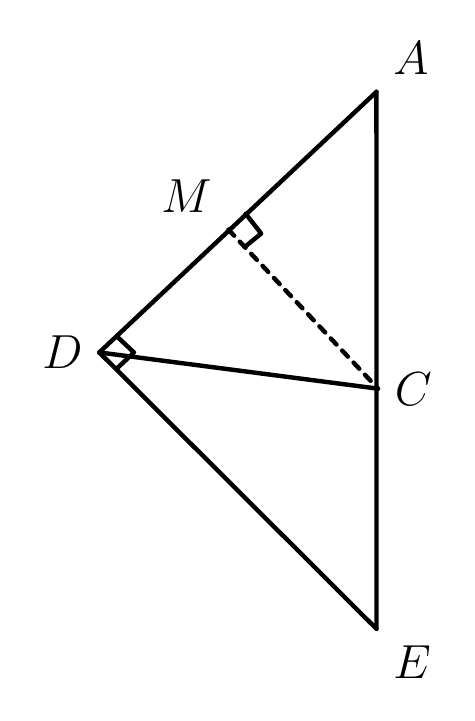
\begin{tikzpicture}[line width=1.6pt, line join=round, line cap=round]
  % Points (pixel -> units, s = 0.01995, y flipped, centre (145,222))
  \coordinate (A) at (1.7599449102106908,3.410058581004571);
  \coordinate (E) at (1.76,-3.41);
  \coordinate (D) at (-1.759944910210691,0.09994141899542885);
  \coordinate (C) at (1.7798979311448941,-0.3600959859217844);
  \coordinate (M) at (-0.11989793114489411,1.6600959859217843);

  % Solid segments
  \draw (A) -- (D);
  \draw (A) -- (E);
  \draw (D) -- (E);
  \draw (D) -- (C);

  % Dashed segment M to C
  \draw[dashed] (M) -- (C);

  % Right-angle mark at M (between MA and MC)
  \draw (0.0990950265308718,1.8611029445230878) -- (0.2955723159471496,1.6100802675567116) -- (0.08557985699500426,1.43807498546007);

  % Right-angle mark at D (between DA and DE, as listed in the GES)
  \draw (-1.5379517972356926,0.30494874479267636) -- (-1.3199518876012335,0.09994906744374046) -- (-1.5379450640070549,-0.10505818882215884);

  % Labels
  \fontsize{16}{19.2}\selectfont
  \node[above right] at (A) {$A$};
  \node[below right] at (E) {$E$};
  \node[left] at (D) {$D$};
  \node[right] at (C) {$C$};
  \node[above left] at (M) {$M$};
\end{tikzpicture}
\end{document}